
    
\subsection{Performance of Layer 5 Prefrontal cortex Pyramidal Neuron on
NeuronUnit tests of model data
agreement}

    \begin{verbatim}[commandchars=\\\{\}]
 \{'value': array(196.875) * pA\}
    \end{verbatim}

    \begin{center}
    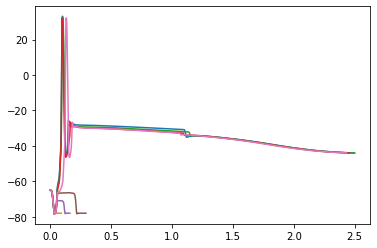
\includegraphics[width=0.7\linewidth]{figures/NU_BBP_fusion_L5PC_files/NU_BBP_fusion_L5PC_3_1.png}
    \end{center}

    \begin{verbatim}
5.74 s +- 34.8 ms per loop (mean +- std. dev. of 7 runs, 1 loop each)
    \end{verbatim}

    \begin{center}
    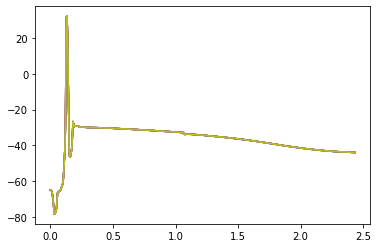
\includegraphics[width=0.7\linewidth]{figures/NU_BBP_fusion_L5PC_files/NU_BBP_fusion_L5PC_4_1.png}
    \end{center}

    \begin{verbatim}
5.74 s +- 64.2 ms per loop (mean +- std. dev. of 7 runs, 1 loop each)
    \end{verbatim}

    \begin{center}
    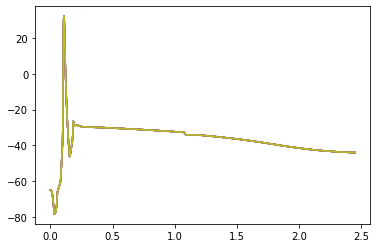
\includegraphics[width=0.7\linewidth]{figures/NU_BBP_fusion_L5PC_files/NU_BBP_fusion_L5PC_4_3.png}
    \end{center}

    \begin{verbatim}[commandchars=\\\{\}]
5.88 s +- 75.3 ms per loop (mean +- std. dev. of 7 runs, 1 loop each)
    \end{verbatim}

    \begin{center}
    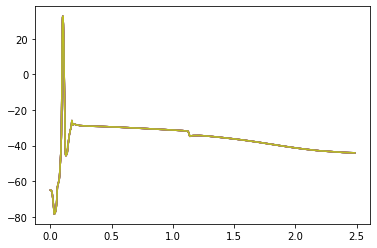
\includegraphics[width=0.7\linewidth]{figures/NU_BBP_fusion_L5PC_files/NU_BBP_fusion_L5PC_4_5.png}
    \end{center}

    \begin{center}
    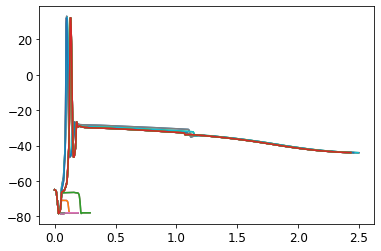
\includegraphics[width=0.7\linewidth]{figures/NU_BBP_fusion_L5PC_files/NU_BBP_fusion_L5PC_6_0.png}
    \end{center}

%    \hypertarget{neocortical-layer-45-pyramidal-cell-test-suite}{%
\subsubsection{Neocortical Layer 4/5 Pyramidal Cell Test
Suite}\label{neocortical-layer-45-pyramidal-cell-test-suite}

\begin{table}[]
\begin{tabular}{|l|l|l|l|l|}
\hline
TestType & experimental-observation & model-prediction& Z-score &  \\ \hline
c & d &  &  &  \\ \hline
  &   &  &  &  \\ \hline
  &   &  &  &  \\ \hline
\end{tabular}
\end{table}    
    
    \begin{verbatim}
  RheobaseTest                                InputResistanceTest  \
    Z = -0.10  Insufficient Data (One of the input values was...   

  TimeConstantTest                                    CapacitanceTest  \
        Z = -0.78  Insufficient Data (One of the input values was...   

  RestingPotentialTest InjectedCurrentAPWidthTest  \
            Z = -1.50                   Z = 7.80   

  InjectedCurrentAPAmplitudeTest InjectedCurrentAPThresholdTest  
                      Z = -1.18                       Z = 1.20  
    \end{verbatim}

    
    
    \begin{verbatim}
observations  213.849583333333 pA    120.672073643411 Mohm   
predictions            196.875 pA  nan kg*m**2/(s**3*A**2)   

observations  15.7342424242424 ms      150.584166666667 pF   
predictions               10.0 ms  nan s**4*A**2/(kg*m**2)   

observations   -68.2481434599156 mV     1.20769387755102 ms   
predictions   -78.04593848610799 mV  0.005377889562759239 s   

observations   80.4351020408164 mV    -42.7357232704403 mV  
predictions   65.34138563793039 mV  -33.093733487773115 mV  
    \end{verbatim}

    
\subsection{Hippocampus CA1 pyramidal cell Cell Test
Suite}\label{hippocampus-ca1-pyramidal-cell-cell-test-suite}

    
    
    \begin{verbatim}
  RheobaseTest                                InputResistanceTest  \
     Z = 0.03  Insufficient Data (One of the input values was...   

  TimeConstantTest                                    CapacitanceTest  \
        Z = -0.67  Insufficient Data (One of the input values was...   

  RestingPotentialTest InjectedCurrentAPWidthTest  \
            Z = -2.62                   Z = 6.67   

  InjectedCurrentAPAmplitudeTest InjectedCurrentAPThresholdTest  
                      Z = -1.71                       Z = 1.88  
    \end{verbatim}
    
    \begin{verbatim}
                       0                        1                    2  \
observations   189.24 pA    107.080327644332 Mohm  24.5021946169772 ms   
predictions   196.875 pA  nan kg*m**2/(s**3*A**2)              10.0 ms   

                                    3                      4  \
observations      89.7960714285714 pF   -65.2261863636364 mV   
predictions   nan s**4*A**2/(kg*m**2)  -78.04593848610799 mV   

                                   5                     6  \
observations     1.31895278450363 ms    86.364525297619 mV   
predictions   0.005377889562759239 s  65.34138563793039 mV   

                                   7  
observations    -47.5985714285714 mV  
predictions   -33.093733487773115 mV  
    \end{verbatim}


